\documentclass[a4paper,11pt]{book}

\usepackage[usenames]{color}
\usepackage{bm}
\usepackage{amsmath}
\usepackage{xspace}
\usepackage{a4wide}
\usepackage{wrapfig}
\usepackage[numbers,comma,sort&compress]{natbib}
\usepackage{graphicx}
\usepackage{xstring}
\usepackage{listings,courier}
%\usepackage{draftcopy}
\usepackage{longtable}
\usepackage{paralist}
%\usepackage{fancyvrb}
%\usepackage{listings}
\usepackage{array}
\usepackage[table]{xcolor}
\usepackage{units}
\usepackage[toc,page]{appendix}
\usepackage{lineno}
\usepackage{makeidx}
\usepackage{palatino}
\usepackage{sidecap}
\usepackage{epstopdf} 


\usepackage[tikz]{bclogo}
% \usepackage[framemethod=tikz]{mdframed}
\usepackage{lipsum}

\usepackage
[pagebackref, %or backref
breaklinks,
colorlinks=true,
linkcolor=webgreen, %defined below
filecolor=webbrown, %defined below
citecolor=webgreen, %defined below
urlcolor=magenta,
pdftitle={VOTCA-CTP manual},
pdfauthor={},
pdfsubject={VOTCA-CTP},
pdfkeywords={charge transport organic semiconductors},
bookmarksopen=false,
pdfpagemode=UseNone]{hyperref}

\usepackage[all]{hypcap}
\usepackage[hyphenbreaks]{breakurl}

\usepackage[T1]{fontenc}
%\usepackage{times}
\usepackage{type1cm}
%\usepackage{showidx}
%\usepackage[draft,color,notref,notcite]{showkeys}

\usepackage{braket}
\usepackage{amssymb}

\usepackage{tikz}
\usetikzlibrary{shapes,shadows,arrows}
\usetikzlibrary{positioning}

\definecolor{bgblue}{RGB}{245,243,253}
\definecolor{ttblue}{RGB}{91,194,224}
\definecolor{webgreen}{rgb}{0,.5,0}
\definecolor{webbrown}{rgb}{.6,0,0}
\definecolor{invisiblegray}{rgb}{.97,0.97,0.97}
\definecolor{mygray}{rgb}{0.86,0.86,0.86}

%\makeindex

\input{newcommands}
\input{gitid}

\usepackage{titlesec}
\titleformat{\chapter}[display]{\normalfont\bfseries}{}{0pt}{\Huge}
\titlespacing*{\chapter}{0pt}{5.5ex plus 1ex minus .2ex}{10pt}

\usepackage[
   a4paper,
   twoside,
   bindingoffset=1cm,
   inner=2.5cm,
   outer=2.5cm,
   top=2.5cm,
   bottom=2.5cm,
   headsep=1.2cm
]{geometry}

\setcounter{secnumdepth}{1} % levels under \section are not numbered
\setcounter{tocdepth}{1}  % levels under \subsection are not listed in the TOC

\begin{document}

%\addtolength{\oddsidemargin}{0cm}
%\addtolength{\evensidemargin}{0cm}
%\addtolength{\textwidth}{0cm}
%\addtolength{\topmargin}{0cm}
%\addtolength{\textheight}{0cm}

\lstset{
  language=XML,
  frame=lines,
  backgroundcolor=\color{invisiblegray},
  basicstyle=\ttfamily\footnotesize,
  identifierstyle=\color{red},
  keywordstyle=\color{blue},
  commentstyle=\color{gray}\rmfamily\itshape,
  mathescape=false
}


\setlength\parindent{15pt}
\frontmatter
\begin{titlepage}

%\center{\fontsize{4cm}{5cm}\selectfont VOTCA-CT}
%\center{\fontsize{1.5cm}{3cm}\selectfont USER MANUAL}

\center{\huge \sc VOTCA-CTP \\ \vspace*{1cm} Charge Transport Simulations}
\vspace*{1cm}
\center{\Large \sc User Manual}

\vspace*{3cm}
\center{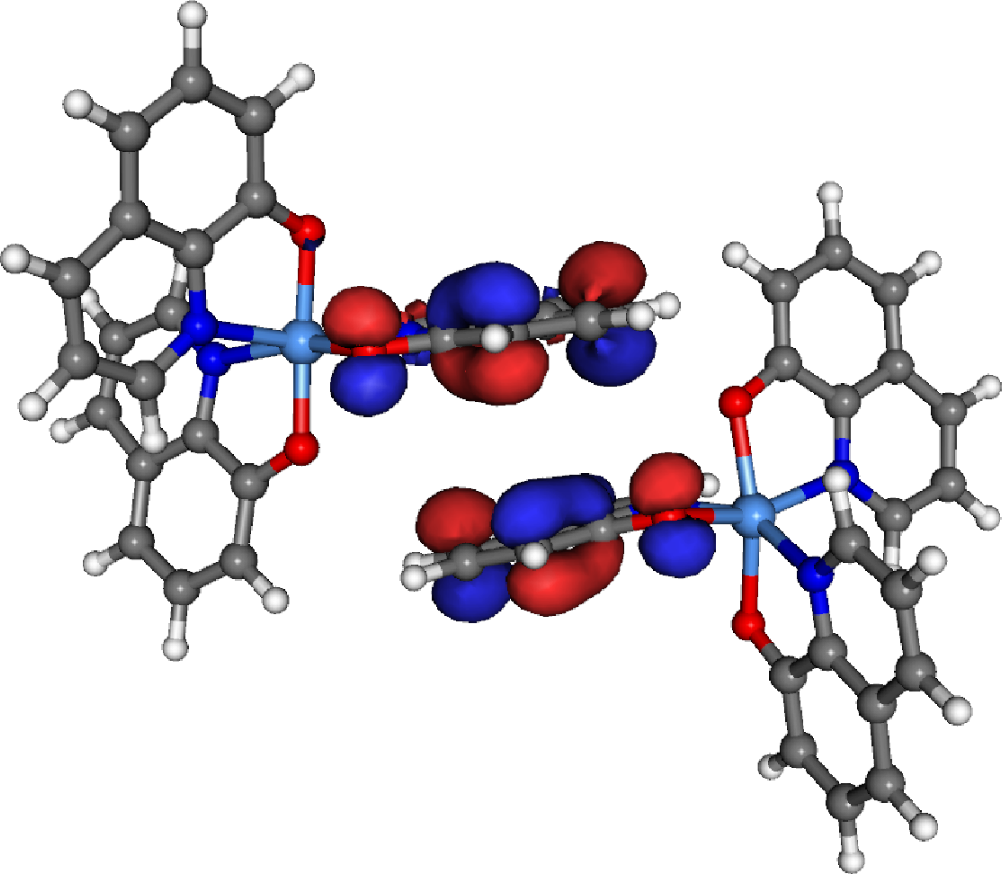
\includegraphics[width=0.6\columnwidth]{fig/logo}}
\vspace*{1cm}
\vfill

%\center{\footnotesize{compiled from: \hgid}}
%\center{\footnotesize{Programs version: \refhgid}}
%\vspace*{1cm}
%\center{
%\large{\copyright \hspace*{0.1cm} VOTCA development team}
%}
\vspace*{0.5cm}
\center{\large{\today}} \\
\vspace*{0.3cm}
\htmladdnormallink{\color{black}\large{www.votca.org}}{http://www.votca.org}
\end{titlepage}

\section*{Disclamer}
Open source projects are made available and contributed to under licenses that include terms that, for the protection of contributors, make clear that the projects are offered ``as-is'', without warranty, and disclaiming liability for damages resulting from using the projects. 

\section*{Citations}
Development of this software depends on academic research grants. If you are using the package, please cite the  following papers \\

\vspace{0.1cm}
\noindent
\cite{poelking_long-range_2016} Long-range embedding of molecular ions and excitations in a polarizable molecular environment, Carl Poelking and Denis Andrienko \\
\htmladdnormallink{  {\itshape J. Chem. Theory Comp.} 12, 4516-4523, 2016}
{http://dx.doi.org/10.1021/acs.jctc.6b00599} \\

\vspace{0.1cm}
\noindent
\cite{kordt_modeling_2016} Modeling of spatially correlated energetic disorder in organic semiconductors,
Pascal Kordt, Denis Andrienko \\
\htmladdnormallink{  {\itshape J. Chem. Theory Comput.}, 12, 36-40, 2016 }
{http://dx.doi.org/10.1021/acs.jctc.5b00764} \\

\vspace{0.1cm}
\noindent
\cite{ruhle_microscopic_2011} Microscopic simulations of charge transport in disordered organic semiconductors, 
Victor R\"uhle, Alexander Lukyanov, Falk May, Manuel Schrader, Thorsten Vehoff, James Kirkpatrick, Bj\"orn Baumeier and Denis Andrienko \\
\htmladdnormallink{  {\itshape J. Chem. Theor. Comp.} 7, 3335, 2011}
{http://dx.doi.org/10.1021/ct200388s} \\

\vspace{0.1cm}
\noindent
\cite{lukyanov_extracting_2010} Extracting nondispersive charge carrier mobilities of organic emiconductors from simulations of small systems, A. Lukyanov, D. Andrienko \\
\htmladdnormallink{  {\itshape Phys. Rev. B}, 82, 193202, 2010}
{http://dx.doi.org/10.1103/PhysRevB.82.193202} \\

\vspace{0.1cm}
\noindent
\cite{baumeier_density-functional_2010}
      Density-functional based determination of intermolecular charge transfer properties for large-scale morphologies, Bj{\"o}rn Baumeier,  James Kirkpatrick, and Denis Andrienko \\
       \htmladdnormallink{  {\itshape  Phys. Chem. Chem. Phys. } 12, 11103, 2010 }{http://dx.doi.org/10.1039/C002337J} \\

\vspace{0.1cm}
\noindent
\cite{ruhle_versatile_2009} Versatile Object-oriented Toolkit for Coarse-graining Applications, 
Victor R\"uhle, Christoph Junghans, Alexander Lukyanov, Kurt Kremer and Denis Andrienko \\
\htmladdnormallink{  {\itshape J. Chem. Theor. Comp.} 5, 3211, 2009}
{http://dx.doi.org/10.1021/ct900369w}

\section*{Development}
The core development is currently taking place at the Max Planck Institute for Polymer Research, Mainz, Germany.

\section*{Copyright}
\votcactp is free software. The entire package is available under the Apache License. For details, check
the LICENSE file in the source code. The \votcactp source code is available on our homepage, \htmladdnormallink{\color{black}www.votca.org}{http://www.votca.org}.

\vfill

\thispagestyle{empty}
\cleardoublepage

{\small \tableofcontents }
\cleardoublepage
\mainmatter

%{\small \printindex }
%\vfill

%\linenumbers

\chapter{Overview}
\label{sec:introduction}

Charge carrier and exciton dynamics in organic semiconductors can often be described as a sequence of charge/exciton transfer reactions between localized states. Transfer rates depend on \slink{sec:transfer_integrals}{electronic coupling elements}, \slink{sec:reorganization}{reorganization energies}, and \slink{sec:site_energies}{site energies}, which vary as a function of molecular positions and orientations. The purpose of the \votcactp package~ is to simplify the computational workflow for charge and exciton transport simulations, which is shown in \Fig{summary}. 

In this workflow, \slink{morphology}{atomistic morphology} is mapped onto \slink{segments}{conjugated segments}  and rigid fragments. If needed, rigid fragments are substituted with the quantum-mechanically optimized copies. The conjugated segments are then used to construct a \slink{neighborlist}{neighbor list}. For each pair of this list an \slink{transfer_integrals}{electronic coupling element}, a \slink{reorganization}{reorganization energy}, a \slink{site_energies}{driving force}, and eventually the \slink{rates}{rate} are evaluated.

Solid-state \slink{sec:site_energies}{ionization energies, electron affinities, and excited state energies} of conjugated segments are calculated perturbatively, as a sum of the gas-phase contribution and electrostatic and polarization interaction with the environment. Coulomb interactions can be evaluated using a cutoff or an aperiodic Ewald summation, available for both the bulk and slab geometries. These calculations require distributed atomic multipoles and polarizabilities for the neutral, cationic (IE), anionic (EA), or excited state.

Electronic \slink{sec:transfer_integrals}{coupling elements} between conjugated segments can be performed by \slink{sec:dipro}{projecting} the dimer orbitals on the respective diabatic states, approximated by the monomer orbitals. Interfaces to \gaussian and, to a lesser extent, to \turbomole are provided to perform these computationally demanding simulations. Alternatively, it is possible to use the fast \slink{sec:izindo}{molecular orbital overlap} method based on the semi-empirical INDO Hamiltonian. This method requires INDO molecular orbitals in the format provided by the \gaussian package.

The \slink{neighborlist}{neighbor list} and \slink{rates}{rates} define a directed graph. The corresponding master equation is solved using the \slink{kmc}{kinetic Monte Carlo} method, which allows to explicitly monitor the charge and exciton dynamics in the system as well as to calculate time- or ensemble averages of occupation probabilities, charge fluxes, correlation functions, and field-dependent mobilities. 

The package is organized in several \slink{sec:programs}{programs} executing \slink{sec:calculators}{calculators}. Results are stored in a \slink{statefile}{sql database} which is also used to restart simulations. In the following we describe individual steps required to perform charge and exciton transport simulations, the format of input and output files, and the complete reference of \slink{sec:programs}{programs} and \slink{sec:calculators}{calculators}, compiled from the installed code. A tutorial is available on the github \hyperref[https://github.com/votca/ctp-tutorials]{github.com/votca/ctp-tutorials}.

\label{sec:wokflow}

\tikzstyle{decision} = [diamond, draw, fill=white]
\tikzstyle{line} = [draw, -stealth, thick]
\tikzstyle{block} = [draw, rectangle, fill=white, text width=0.6\linewidth]
\tikzstyle{smallblock} = [draw, rectangle, fill=white, text width=0.4\linewidth]
\tikzstyle{info} = [text width=0.35\linewidth]
\tikzstyle{smallinfo} = [text width=0.25\linewidth]
\tikzstyle{biginfo} = [text width=0.9\linewidth]

\begin{figure}
\centering
\newcommand{\vgap}{0.5cm}
\begin{scriptsize}
\noindent\begin{tikzpicture}

\node [block] (mapping) {
{\bf Mapping, generation of the sql database}\\
Converts and partitions atomistic \gromacs trajectory \vskip 0.1cm
{\noindent  \cmdmap} \\
Useful tools: \calc{pdb2map}

\vskip 0.1cm };

\node[smallinfo, left=0.0 of mapping] (input) {{\bf Input files:}\\\texttt{conf.gro}\\\,\hskip 0.1cm\gromacs trajectory\\\texttt{topol.tpr}\\\hskip0.1cm\gromacs topology\\\texttt{\xmlcsg}\\\hskip0.1cm mapping and energies\\\texttt{options.xml}\\\hskip0.1cm options for \slink{sec:calculators}{calculators}\vskip 0.2cm {\bf Output files:}\\\texttt{\sqlstate}\\\hskip0.1cm \sqlite database file for\\\hskip0.1cm data transfer between\\\hskip0.1cm modules};

\node [block, below=\vgap of mapping] (nbl) {{\bf Neighbor list}\\Indentifies close molecular pairs between which charge transfer rates will be calculated \vskip 0.1cm
{\noindent \cmdnbl}
\vskip 0.1cm};


\node [block, below=\vgap of nbl] (site_energies) {{\bf Site energies}\\Calculates electrostatic and polarization contribution to site energies \vskip 0.1cm
{\noindent  \cmdemlt} };

\node [block, below=\vgap of site_energies] (int_energies) {{\bf Internal site and reorganization energies}\\Imports internal site energy (IP, EA) and reorganization energies for charging and discharging to \sqlstate \vskip 0.1cm
{\noindent  \cmdeint}
\vskip 0.1cm};


% above right=0.7cm and 4cm of A
\node[decision, below=\vgap of int_energies](decision1){Transfer integrals};

%\node (AuxNode01) [text width=6em, below of = decision1, node distance=7em ] {};

\node [smallblock, below left=\vgap of decision1] (DFT_TI) {{\bf Monomers with DFT}\\Calculate the relevant transport orbitals of monomers \vskip 0.1cm
{ \cmdedft \job\, ''\wrt \run'' }};

\node [smallblock, below=\vgap of DFT_TI] (DFT_TI2) {{\bf Transfer integrals with DFT}\\Calculate electronic coupling elements for all pairs in the neighbor list \vskip 0.1cm
{ \cmdidft \job\, ''\wrt \run \rd'' }
\vskip 0.1cm};

\node [smallblock, below right=\vgap of decision1] (DFT_ZINDO) {{\bf Transfer integrals with ZINDO}\\Calculate electronic coupling elements for all pairs in the neighbor list  \vskip 0.1cm
{\noindent  \cmdizindo }
\vskip 0.1cm};


\node[info, below=0.2cm of DFT_ZINDO] (ti_info) {{One can choose between quantum-chemical (computationally expensive) or semi-empirical (fast, but not always sufficiently accurate) evaluation of transfer integrals.}};

\node (AuxNode01) [below=\vgap of DFT_TI2, xshift=0.25\linewidth] {};


\node [block, below=\vgap of DFT_TI2, xshift=0.275\linewidth] (outer_reorg) {{\bf Outersphere reorganization energies}\\Contribution to reorganization of surrounding molecules due to polarization. (optional for Marcus rates)  \vskip 0.1cm
{\noindent  \cmdouter}
\vskip 0.1cm};

\node [block, below=\vgap of outer_reorg] (rates) {{\bf Charge transfer rates}\\Calculates rates for charge transfer among all pairs in the neighborlist \vskip 0.1cm
{\noindent \cmdrates}
};

\node [block, below=\vgap of rates] (kmc) {{\bf Charge dynamics via kMC}\\Hopping of charge carriers simulated via kinetic Monte Carlo \vskip 0.1cm
{\noindent \cmdkmc }
};

\node [biginfo, below=\vgap of kmc] (calc) {{\noindent Get list of available calculators: \ctprun/\ctpparallel/\kmcrun  \texttt{ -l}}\\ Get help and list of options for a calculator: \ctprun/\ctpparallel/\kmcrun  \texttt{ -d }\calc{neighborlist}};

\path [line] (mapping) -- (nbl);
\path [line] (nbl) -- (site_energies);
\path [line] (site_energies) -- (int_energies);
\path [line] (int_energies) -- (decision1);
\path [line] (DFT_TI) -- (DFT_TI2);
\path [line] (decision1) -| node[yshift=0.5em, xshift=1em] {DFT} (DFT_TI);
\path [line] (decision1) -| node[yshift=0.5em, xshift=-1em] {ZINDO} (DFT_ZINDO);
\path [line] (DFT_TI2.east) -| (outer_reorg.north);
\path [line] (DFT_ZINDO.west) -| (outer_reorg);
\path [line] (outer_reorg) -- (rates);
\path [line] (rates) -- (kmc);
\end{tikzpicture}


\end{scriptsize}
\caption{A cheat sheet for charge and exciton transport simulations. }
\label{fig:summary}
\end{figure}

	

% MORPHOLOGY PARTITIONING
\chapter{Morphology}
\label{sec:morphology}

There is no generic recipe on how to predict a large-scale atomistically-resolved morphology of an organic semiconductor. The required methods are system-specific: for ultra-pure crystals, for example, density-functional methods can be used provided the crystal structure is known from experiment. For partially disordered organic semiconductors, however, system sizes much larger than a unit cell  are required. Classical molecular dynamics or Monte Carlo techniques are then the methods of choice. 

In molecular dynamics, atoms are represented by point masses which interact via empirical potentials prescribed by a force-field. Force-fields are parametrized for a limited set of compounds and their refinement is often required for new molecules. In particular, special attention shall be paid to torsion potentials between successive repeat units of conjugated polymers or between functional groups and the $\pi$-conjugated system. First-principles methods can be used to characterize the missing terms of the potential energy function. 

Self-assembling materials, such as soluble oligomers, discotic liquid crystals, block copolymers, partially crystalline polymers, etc., are the most complicated to study. The morphology of such systems often has several characteristic length scales and can be kinetically arrested in a thermodynamically non-equilibrium state. For such systems, the time- and length-scales of atomistic simulations might be insufficient to equilibrate or sample desired morphologies. In this case, systematic coarse-graining can be used to enhance sampling~\cite{ruhle_versatile_2009}. Note that the coarse-grained representation must reflect the structure of the atomistic system and allow for back-mapping to the atomistic resolution.

Here we assume that the topology and the coordinates of all atoms are known. \votcactp can read standard \gromacs topology files. Custom definitions of \slink{sec:atomistic}{atomistic topology} via \xml files are also possible.


\section{Conjugated segments and rigid fragments}
\label{sec:segments}

\begin{figure}
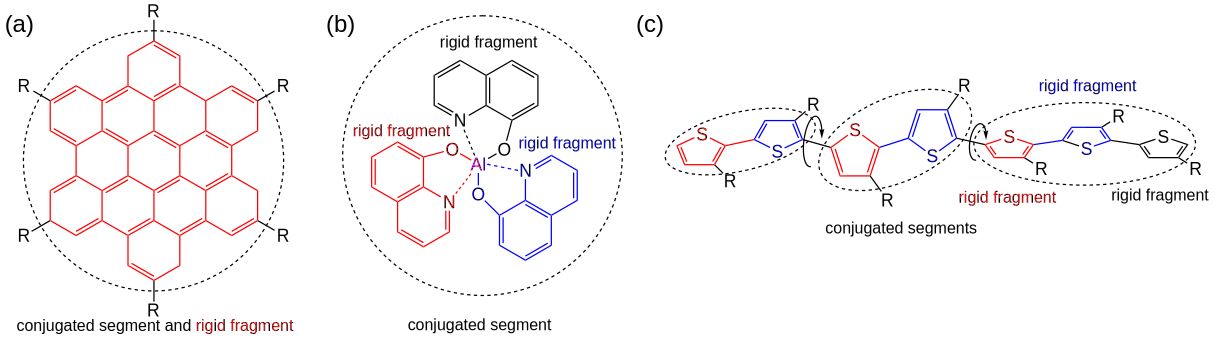
\includegraphics[width=\linewidth]{fig/fragment_segment}
\caption{The concept of conjugated segments and rigid fragments. Dashed lines indicate conjugated segments while colors denote rigid fragments. (a) Hexabenzocoronene: the $\pi$-conjugated system is both a rigid fragment and a conjugated segment. (b) \Alq: the Al atom and each ligand are rigid fragments while the whole molecule is a conjugated segment. (c) Polythiophene: each repeat unit is a rigid fragment. A conjugated segment consists of one or more rigid fragments. One molecule can have several conjugated segments.}
\label{fig:segment}
\end{figure}

With the morphology at hand, the next step is partitioning the system on hopping sites\index{hopping site}, or conjugated segments\index{conjugated segment}, and calculating charge transfer rates between them. Physically intuitive arguments can be used for the partitioning,  which reflects the localization of the wave function of a charge. For most organic semiconductors, the molecular architecture includes relatively rigid, planar $\pi$-conjugated systems, which we will refer to as rigid fragments. A conjugated segment can contain one or more of such rigid fragments, which are linked by bonded degrees of freedom. The dynamics of these degrees of freedom evolves on timescales much slower than the frequency of the internal promoting mode. In some cases, e.g. glasses, it can be `frozen' due to non-bonded interactions with the surrounding molecules.

To illustrate the concept of conjugated segments and rigid fragments, three representative molecular architectures are shown in \fig{segment}. The first one is a typical discotic liquid crystal, hexabenzocoronene. It consists of a conjugated core to which side chains are attached to aid self-assembly and solution processing. In this case the orbitals localized on side chains do not participate in charge transport and the conjugated $\pi$-system is both, a rigid fragment and a conjugated segment. 
%
In \Alq, a metal-coordinated compound, a charge carrier is delocalized over all three ligands. Hence, the whole molecule is one conjugated segment. Individual ligands are relatively rigid, while energies of the order of $k_\text{B}T$ are sufficient to reorient them with respect to each other. Thus the Al atom and the three ligands are rigid fragments.
%
In the case of a conjugated polymer, one molecule can consist of several conjugated segments, while each backbone repeat unit is a rigid fragment. Since the conjugation along the backbone can be broken due to large out-of-plane twists between two repeat units, an empirical criterion, based on the dihedral angle, can be used to partition the backbone on conjugated segments~\cite{ruhle_multiscale_2010}. However, such intuitive partitioning is, to some extent, arbitrary and shall be validated by other methods~\cite{vukmirovic_charge_2008,vukmirovic_charge_2009,mcmahon_ad_2009}. 

After partitioning, an additional step is often required to remove bond length fluctuations introduced by molecular dynamics simulations, since they are already integrated out in the derivation of the rate expression. This is achieved by substituting respective molecular fragments with  rigid, planar $\pi$-systems\index{rigid fragment} optimized using first-principles methods. Centers of mass and gyration tensors are used to align rigid fragments, though a custom definition of local axes is also possible. Such a procedure also minimizes discrepancies between the force-field and first-principles-based ground state geometries of conjugated segments, which might be important for calculations of electronic couplings, reorganization energies, and intramolecular driving forces. 

\section{Mapping file}
\label{sec:xmlmap}
The partitioning of the system on conjugated segments and rigid fragments is specified in the mapping file, \xmlcsg. Using this input, \ctpmap converts an atomistic configuration into a configuration with conjugated segments and rigid fragments and stores it in a \slink{statefile}{state file}:
%
\votcacommand{Mapping using the \gromacs topology and trajectory}{\cmdmap}
%
\ctpmap reads in the \gromacs topology from \topology, trajectory from \trajectory, definitions of conjugated segments and rigid fragments from \xmlcsg and outputs coordinates of segments and fragments to the state file, \sqlstate. After this step, dimensions of the simulation box, atom coordinates, etc, are stored in the \slink{statefile}{state file}.

\attention{\votcactp requires a wrapped \gromacs trajectory, i.~e., all molecules should be whole in the snapshot.}  

Mapping file provides three different representations of the molecule: (i) partitioning on conjugated segments and rigid fragments (mdatoms), (ii) QM-optimized geometry (qmatoms), and (iii) partitioning on electrostatic multipoles (mpoles). An example of \xmlcsg for a \dcvt molecule is shown in listing~\ref{list:map}. 

% Define new language for listings.
\lstdefinelanguage{MXML} {
   basicstyle=\ttfamily\tiny,
   sensitive=true,
   morecomment=[s][\color{gray}\rmfamily\itshape]{<!--}{-->}, 
   showstringspaces=false,
   numberstyle=\tiny,
   numberblanklines=true,
   showspaces=false,
   breaklines=true,
   showtabs=false,
   alsoletter={:},
   keywords = [1]
   { topology,molecules,molecule,name,mdname,segments,segment,fragments,fragment,mdatoms,qmatoms,mpoles,localframe,localframe_mps,orbitals,weights,weights_mps,virtual_mps,qmcoords,torbital_h, torbital_e, multipoles_n, multipoles_h, multipoles_e, map2md, U_cC_nN_h, U_nC_nN_h, U_cN_cC_h},
   keywordstyle={[1]\color{blue}},
}

\newpage
\lstinputlisting[
 language=MXML,
 label=list:map,
 caption={Examle of \xmlcsg for \dcvt. Each rigid fragment (coarse-grained bead) is defined by a list of atoms. Atom numbers, names, and residue names should correspond to those used in \gromacs topology (see the corresponing listing \ref{list:pdb} of the pdb file).}]%
{./input/dcv2t/map.xml}
\vfill

The corresponding atom numbers, names, residue numbers, and residue types of  \dcvt are shown in fig.~\ref{fig:dcv2t} and in listing~\ref{list:pdb}. \dcvt has two thiophene (THI) and two dicyanovinyl (NIT) residues, which are used to partition the molecule on four rigid fragments. Since the molecule is planar, it is represented by one conjugated segment.

\newpage
\begin{figure}[ht]
\centering
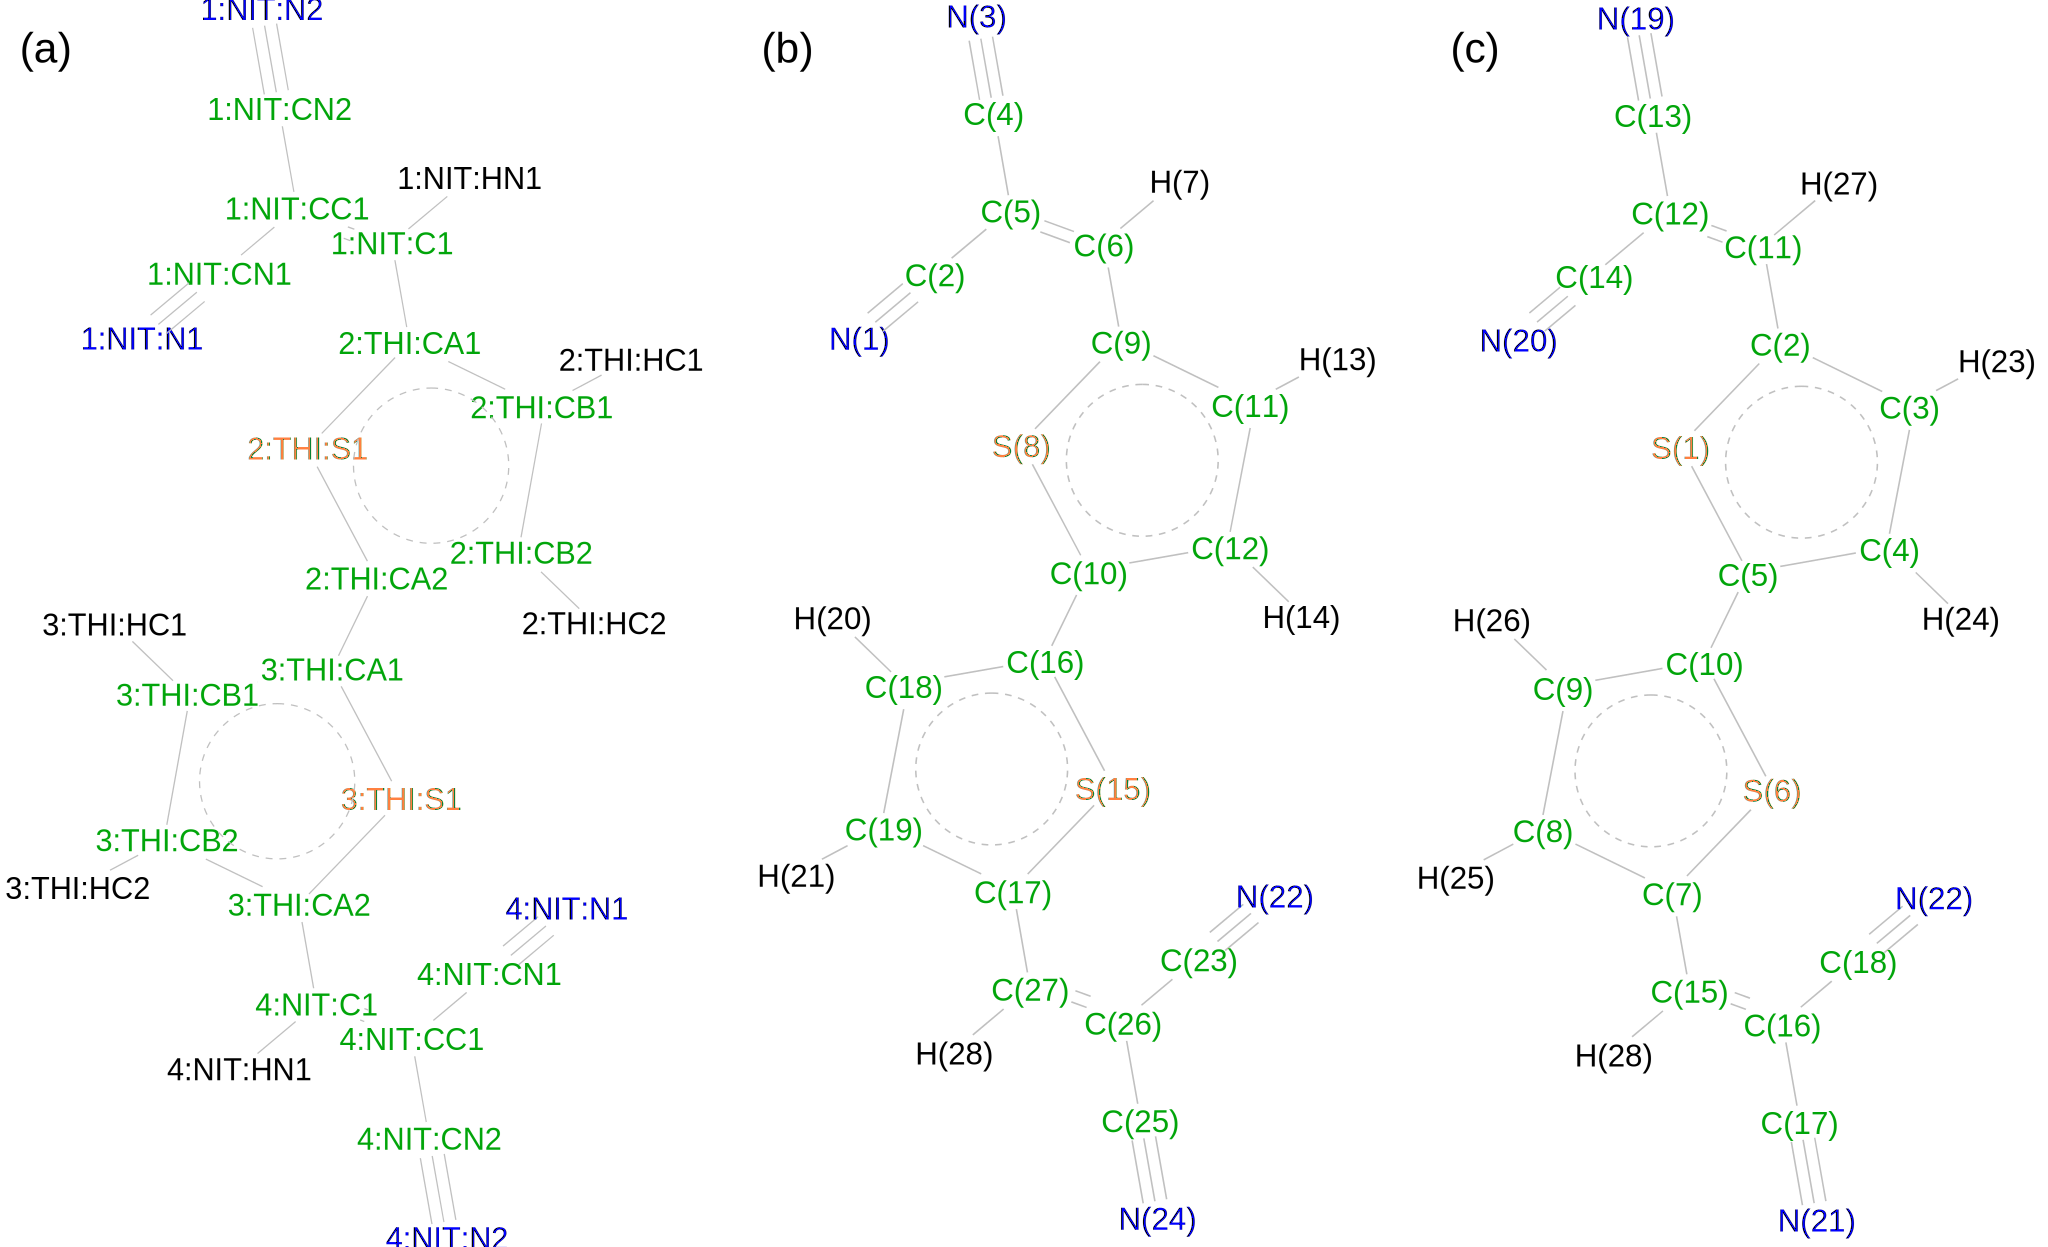
\includegraphics[width=0.8\textwidth]{./fig/dcv2t}
\caption{\small (a) \dcvt with atoms labelled according to \texttt{residue\_number:residue\_name:atom\_name}. 
There are four residues and two residue types: thiophene (THI) and dicyanovinyl (NIT). The corresponding pdb file is shown in listing~\ref{list:pdb}. Atom numbering is used to split conjugated segments on rigid fragments and to link atomistic (b) and quantum-mechanical (c) descriptions.}
\label{fig:dcv2t}
\end{figure}

\lstinputlisting[
  language=XML,
  basicstyle=\ttfamily\footnotesize,
  stringstyle=\ttfamily\footnotesize,
  showstringspaces=false,
  frame=lines,
  label=list:pdb, 
  morekeywords={HETATM,THI,NIT},
  caption={ pdb file of \dcvt.}]%
{./input/dcv2t/dcv2t.pdb}
\vfill

% PRACTICAL ADVICE
Generation of the mapping file can be semi-automatized if the atom order, residue numbering and types in the atomistic morphology reflect partitioning on rigid fragments.  This can be achieved already at the stage of preparing input files for atomistic simulations, by insuring that rigid fragments in the pdb files of all segments have   different residue types and numbers. A \dcvt pdb file, shown in listing~\ref{list:pdb}, is an example of such partitioning, where residue types (NIT and THI) and residue numbers (5-th column, from 1 to 4) uniquely define rigid fragments.

Such pdb files can be used to generate templates of \gromacs topologies, with the help of the \calc{pdb2top} tool,
\votcacommand{Creating a topol.top from a pdb file}{\small \ctptools \sql \sqlstate \exe \calc{pdb2top} }
and the mapping file, using the \calc{pdb2map} tool, 
\votcacommand{Creating a \xmlcsg from a pdb file}{\small \ctptools \sql \sqlstate \exe \calc{pdb2map} }

Both files need further refinement, but this procedure helps to avoid typos and inconsistencies between atomistic and coarse-grained morphologies.


\section{Validating the mapping}
\label{sec:ctp_dump}
% CHECKS
In order to visually check the mapping one can use calculator \calc{trajectory2pdb} of the \ctpdump program.
%
\votcacommand{Writing a mapped trajectroy with \ctpdump}{\small \ctpdump \sql \sqlstate \exe \calc{trajectory2pdb} }
%
\ctpdump reads in the state file created by \ctpmap and outputs two trajectory files corresponding to the original and rigidified atom coordinates. To check the mapping, you can superimpose the three outputs: original atomistic, atomistic stored in the state file, and rigidified according to the ground state geometries. This can be done with, e.g., {\tt VMD}. Note that \ctpdump can also output the list of segments, 
\votcacommand{List of conjugated segments}{\small \ctpdump \sql \sqlstate \exe \calc{segments2xml} }

Alternatively, \calc{tdump} of \ctprun reads in the state file and appends the coordinates to QM.pdb and MD.pdb. Make sure to delete old QM.pdb and MD.pdb if you want to create a new image.
\label{sec:tdump}
\votcacommand{Writing a mapped trajectory with \calc{tdump} }{\small \ctprun \sql \sqlstate \opt \xmloptions \exe \calc{tdump} }




\section{Custom topologies}

\gromacs configurations and binary topologies (\texttt{topology.tpr}) can be used directly by the \ctpmap program. In this case residue and atom names should be used to specify the \slink{xmlmap}{coarse-grained topology} and \slink{xmlsegments}{conjugated segments}. 

A custom topology can also be defined using an \xml file. It is also possible to partially overwrite the information provided in, for example, \gromacs topology file. 

%We will illustrate how to create a custom topology file using \dcvt. 

\input{input/topology_atomistic}
\input{input/topology_coarsegrained}
\input{input/topology_conjseg}
\chapter{Neighbor list}
\label{sec:neighborlist}

A list of neighboring conjugated segments, or neighbor list\index{neighbor list}, contains all pairs of conjugated segments for which \slink{sec:transfer_integrals}{coupling elements}, \slink{sec:reorganization}{reorganization energies}, \slink{sec:site_energies}{site energy differences}, and \slink{sec:rates}{rates} are evaluated.

Two segments are added to this list if the distance between centers of mass of any of their rigid fragments is below a certain cutoff. This allows neighbors to be selected on a criterion of minimum distance of approach rather than center of mass distance, which is useful for molecules with anisotropic shapes.

The neighbor list can be generated from the atomistic trajectory by using the \calc{neighborlist} \calculator. This calculator requires a cutoff, which can be specified in the \xmloptions file. The list is saved to the \sqlstate file:
\votcacommand{Generating a neighbor list}{\cmdnbl}

Sometimes it is convenient to filter the rigid fragments, for example if a conjugated segment has alkyl side chains and we do not want to add a pair of molecules which have conjugated cores far apart but side chains close to each other. In this case one can provide a list of ``active'' fragments. The search algorithm will only look at the pairs of segments, for which these fragments are located closer than the specified cutoff.

It can also happen that a completely custom neighbor list is required. An external list can be imported from a file which has the format pairID, segment1ID, segment2ID, segment1Type, segment2Type, e.g.,
\lstset{language=XML}
\begin{lstlisting}
1  1 2 DCV DCV  
2  1 3 DCV DCV     
3  2 3 DCV DCV 
\end{lstlisting}


% REORGANIZATION ENERGY
\input{theory/reorganization_energy}

% SITE ENERGIES
\input{theory/energetic_disorder}
\input{theory/gdma}
\input{theory/thole}
\section{Ewald sums}
\label{sec:ewald}
\index{Long-range interactions}
\index{site energy!Ewald}

This section is a practical guide for doing electrostatic calculations in slabs using aperiodic Ewald scheme described in \cite{poelking_long-range_2016}.

First, you will need to generate the required quantum mechanical reference, comprising molecular charge density and polarizability for all charge states (neutral, cationic, anionic). For example, you can use  GAUSSIAN to do this:
 \begin{verbatim}
...
#p b3lyp/6-31+g(d,p) pop(full,chelpg) polar(dipole) nosymm test
...
 \end{verbatim}

Afterwords, you have to generate all required {\em mps}-files with distributed multipoles and polarizabilities.  The options file should point to the QM {\em log}-files, as well as contain the target molecular polarizability tensor in upper-diagonal order $xx$ $xy$ $xz$ $yy$ $yz$ $zz$ in units of \AA$^3$.
\begin{verbatim}
$ ctp_tools -e log2mps -o options.xml
$ ctp_tools -e molpol -o options.xml

<options>
    <log2mps>
        <package>gaussian</package>
        <logfile>input.log</logfile>
        <mpsfile></mpsfile>
    </log2mps>
    <molpol>
        <mpsfiles>
            <input>input.mps</input>
            <output>output.mps</output>
            <polar>output.xml</polar>
        </mpsfiles>
        <induction>
            <expdamp>0.39000</expdamp>
            <wSOR>0.30000</wSOR>
            <maxiter>1024</maxiter>
            <tolerance>0.00001</tolerance>
        </induction>
        <target>
            <optimize>true</optimize>
            <molpol>77 0 0 77 0 77</molpol>
            <tolerance>0.00001</tolerance>
        </target>
    </molpol>
</options>
  \end{verbatim}
 
Next, generate the {\it mps} table, which relates the state of the molecule (neutral, cation, anion) with a corresponding electrostatic representation. This  is provided by the {\em stateserver}. The resulting output file has the default name ``mps.tab'':
\begin{verbatim}
$ ctp_run -e stateserver -o options.xml -f state.sql

<options>
    <stateserver>
        <keys>mps</keys>
    </stateserver>
</options>
\end{verbatim}

Next, generate the job file. This job file lists the electrostatic configurations that are to be investigated. It can either be composed by hand or generated automatically from the {\em sql} file via the {\em jobwriter}, which at present takes either ``mps.chrg'', ``mps.single'' or ``mps.ct'' as key, where the latter resorts to a neighbor list. The resulting {\em xml}-file has the default name ``jobwriter.mps.chrg.xml''.
\begin{verbatim}
$ ctp_run -e jobwriter -o options.xml -f state.sql

<options>
    <jobwriter>
        <keys>mps.chrg</keys>
	 <single_id>10</single_id>
	 <cutoff>3</cutoff>
    </jobwriter>
</options> 
\end{verbatim}

The input string in the job file for the long-range corrected calculators has the same format as for the {\em xqmultipole} calculator, ``id1:name1:mps1 id2:name2:mps2 ...''. See sample below.
\begin{verbatim}
 <jobs>
    <job>
        <id>1</id>
        <tag>1e:2h</tag>
        <input>1:spl:MP_FILES/spl_e.mps 2:spl:MP_FILES/spl_h.mps</input>
        <status>AVAILABLE</status>
    </job>
    <job>
        ...
    </job>
    ...
</jobs>
\end{verbatim}

Next, generate the {\em ptop}-file that stores the induction state of the neutral {\em background}. The responsible {\em ewdbgpol} calculator can be run in a threaded fashion, depending on system size. The resulting {\em ptop}-file has the default name ``bgp\_main.ptop''. 
\begin{verbatim}
$ ctp_run -e ewdbgpol -o options.xml -f state.sql -t 8

<options>
    <ewdbgpol>
        <multipoles>system.xml</multipoles>
        <control>
            <mps_table>mps.tab</mps_table>
            <pdb_check>1</pdb_check>
        </control>
        <coulombmethod>
            <method>ewald</method>
            <cutoff>6</cutoff>
            <shape>xyslab</shape>
        </coulombmethod>
        <polarmethod>
            <method>thole</method>
            <wSOR_N>0.350</wSOR_N>
            <aDamp>0.390</aDamp>
        </polarmethod>
        <convergence>
            <energy>1e-05</energy>
            <kfactor>100</kfactor>
            <rfactor>6</rfactor>
        </convergence>
    </ewdbgpol>
</options>
\end{verbatim}

Finally, run the energy computation using {\em pewald3d}. This job calculator is wrapped by the ctp\_parallel executable, which allows for communication between different processes via the job and state file. Unfortunately, communication, though guarded by a file lock, may fail on some architectures in the event of frequent accesses to the job file. This frequency can be controlled by the -c/--cache argument, which defines the number of jobs that are loaded in {\em one} batch by a specific process/node.
\begin{verbatim}
$ ctp_parallel -e pewald3d -o options.xml -f /absolute/path/to/state.sql -s 0 -t 8 -c 40

<options>
    <ewald>
        <jobcontrol>
            <job_file>/absolute/path/to/jobs.xml</job_file>
        </jobcontrol>
        <multipoles>
            <mapping>system.xml</mapping>
            <mps_table>mps.tab</mps_table>
            <polar_bg>bgp_main.ptop</polar_bg>
            <pdb_check>0</pdb_check>
        </multipoles>
        <coulombmethod>
            <method>ewald</method>
            <cutoff>8</cutoff>
            <shape>xyslab</shape>
            <save_nblist>false</save_nblist>
        </coulombmethod>
        <polarmethod>
            <method>thole</method>
            <induce>1</induce>
            <cutoff>4</cutoff>
            <tolerance>0.001</tolerance>
            <radial_dielectric>4.0</radial_dielectric>
        </polarmethod>
        <tasks>
            <calculate_fields>true</calculate_fields>
            <polarize_fg>true</polarize_fg>
            <evaluate_energy>true</evaluate_energy>
            <apply_radial>false</apply_radial>
        </tasks>
        <coarsegrain>
            <cg_background>false</cg_background>
            <cg_foreground>false</cg_foreground>
            <cg_radius>3</cg_radius>
            <cg_anisotropic>true</cg_anisotropic>
        </coarsegrain>
        <convergence>
            <energy>1e-05</energy>
            <kfactor>100</kfactor>
            <rfactor>6</rfactor>
        </convergence>
    </ewald>
</options>
\end{verbatim}

Parse the output. The results from the computation are stored in the same job file that was supplied to the calculator. The key data is provided in the {\em output/summary} section and consists of the electrostatic and induction contributions {\em output/summary/eindu} and {\em output/summary/estat}. Note that only configuration energy {\em differences} carry meaning. The parsing is best done by script, as the ``-j/--jobs read'' option for pewald3d is not yet implemented.

\begin{verbatim}
 <jobs>
    <job>
        <id>1</id>
        <tag>1e:2h</tag>
        <input>1:spl:MP_FILES/spl_e.mps 2:spl:MP_FILES/spl_h.mps</input>
        <status>COMPLETE</status>
        <host>thop76:5476</host>
        <time>17:22:56</time>
        <output>
            <summary>
                <type>neutral</type>
                <xyz unit="nm">-0.1750000 -0.1750000 -5.4250000</xyz>
                <total unit="eV">-3.2112834</total>
                <estat unit="eV">-2.3753255</estat>
                <eindu unit="eV">-0.8359579</eindu>
            </summary>
            <terms_i>
                <F-00-01-11>-3.32999e+00 -3.32481e-01 +4.06829e-02</F-00-01-11>
                <M-00-11--->+1.33689e-01 +4.74490e-01</M-00-11--->
                <E-PP-PU-UU>-2.37533e+00 -7.37812e-01 -2.73212e-18</E-PP-PU-UU>
            </terms_i>
            <terms_o>
                <R-pp-pu-uu>-1.89357e-01 = +2.69583e-08 ...</R-pp-pu-uu>
                <K-pp-pu-uu>-7.31703e-03 = -2.69583e-08 ...</K-pp-pu-uu>
                <O-pp-pu-uu>+0.00000e+00 = +0.00000e+00 ...</O-pp-pu-uu>
                <J-pp-pu-uu>+5.14048e-04 = -2.99187e-17 ...</J-pp-pu-uu>
                <C-pp-pu-uu>+1.51186e-03 = +0.00000e+00 ...</C-pp-pu-uu>
                <Q-pp-pu-uu>+0.00000e+00 = +0.00000e+00 ...</Q-pp-pu-uu>
            </terms_o>
            <shells>
                <FGC>1874</FGC>
                <FGN>1874</FGN>
                <MGN>54429</MGN>
                <BGN>36</BGN>
                <BGP>52</BGP>
                <QM0>2</QM0>
                <MM1>1872</MM1>
                <MM2>0</MM2>
            </shells>
            <timing>
                <t_total unit="min">5.29</t_total>
                <t_wload unit="min">0.00 2.24 0.88 2.18</t_wload>
            </timing>
        </output>
    </job>
    <job>
	     ...
    </job>
	 ...
</jobs>
    
\end{verbatim}


% ELECTRONIC COUPLINGS
\input{theory/electronic_couplings}

% RATES
\input{theory/rate}

% KINETIC MONTE CARLO
\input{theory/kmc}
\input{theory/nondispersive}

% ANALYSIS
\input{theory/analysis}
\input{theory/correlations}

\chapter{Input and output files}
\label{sec:io}

\input{input/orbitals_zindo}
\input{input/header_edft}
\input{input/header_idft}
\input{input/output_dft}
\input{input/statefile}

\input{reference/reference}

\appendix
%\input{appendix/moo_standalone}

\nolinenumbers

\bibliographystyle{short}
{\footnotesize \bibliography{manual} }

\end{document} 
